%%%%%%%%%%%%%%%%%%%%%%%%%%%%%%%%%%%%%%%%%%%%%%%%%%%%%%%%%%%%%%%%%%%%%%%%%%%%%%%%
\section{Calibrated and Uncalibrated Photometric Stereo}\label{sec:bg_ps}
%%%%%%%%%%%%%%%%%%%%%%%%%%%%%%%%%%%%%%%%%%%%%%%%%%%%%%%%%%%%%%%%%%%%%%%%%%%%%%%%
The original Photometric Stereo (PS)~\cite{woodham1980photometric} problem
is a relaxation of Shape-from-Shading (SfS) in which multiple images under
known, varying illumination are required. The most common form of
PS~\cite{woodham1980photometric} assumes a Lambertian BRDF and time-multiplexed 
illumination. Time-multiplexed illumination implies that the input images
are lit under novel illumination patterns and the images are acquired 
sequentially with a time dela between each capture. Given the natural
ill-posedness of the Lambertian SfS problem (as shown by
\labelcref{eq:bg_sfs_least_squares_lambert}), PS solves the problem by requiring
3 or more images under known illumination. Given 3+ images,
\cref{eq:bg_sfs_least_squares_lambert} becomes stable and an albedo per pixel 
may also be recovered. More precisely, a surface normal and diffuse albedo
may be recovered per pixel by solving a linear least squares problem:
%%%%%%%%%%%%%%%%%%%
\begin{equation}\label{eg:bg_ps_lambertian_ls}
	 \min_{\bb{\tilde{N}}} \lVert \bb{X} - \bb{\tilde{N}} \bb{S} \rVert_F
\end{equation}
%%%%%%%%%%%%%%%%%%%
following the notation from \cref{eq:bg_sfs_least_squares_lambert},
assuming $n$ input images of the same width and height ($d$ total pixels) and
$\bb{X} = [\bb{I}_1, \ldots, \bb{I}_n] \in \R^{d \times n}$, 
$\bb{S} = {[\bb{s}_1, \ldots, \bb{s}_n]}^T \in \R^{3 \times n}$ and
$\bb{\tilde{N}} = \nobreak {[\rho_{\smallsub{d}}(x_1, y_1)\bb{n}(x_1, y_1), \ldots, \rho_{\smallsub{d}}(x_w, y_h)\bb{n}(x_w, y_h)]}^T \in \R^{d \times 3}$ 
is the normal matrix scaled by the diffuse
albedo. \cref{eg:bg_ps_lambertian_ls} is solved via a
pseudoinverse as $\bb{\tilde{N}} = \bb{X} \bb{S}^{\dagger}$ and the norm of each
row of $\bb{\tilde{N}}$ recovers the diffuse albedo,
${\rho_{\smallsub{d}}}^i = \norm{\bb{\tilde{n}}^i}$ 
where $i$ is an index into the image space and thus $i \in [1, d]$ 
is the $i$th pixel and
$\bb{\tilde{n}}^i = \bb{\tilde{N}}_{i\ast}^T \in \R^{3 \times 1}$.
Similarly, the unit normals are recovered by
$\bb{\tilde{n}}^i = \frac{\bb{\tilde{n}}^i}{\norm{\bb{\tilde{n}}^i}}$.
%%%%%%%%%%%%%%%%%%%%%%%%%%%%%%%%%%%%%%%%
\begin{figure}[t]
	\centering
	\hspace*{\fill}
	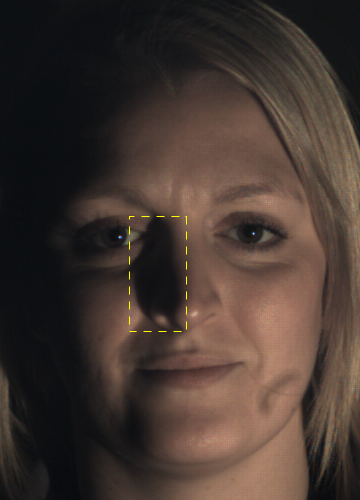
\includegraphics[height=2in]{background/images/photoface0} \hfill
	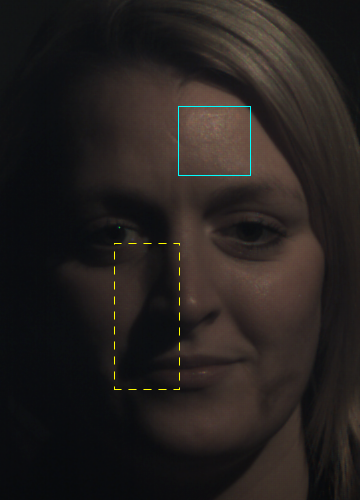
\includegraphics[height=2in]{background/images/photoface1} \hfill
	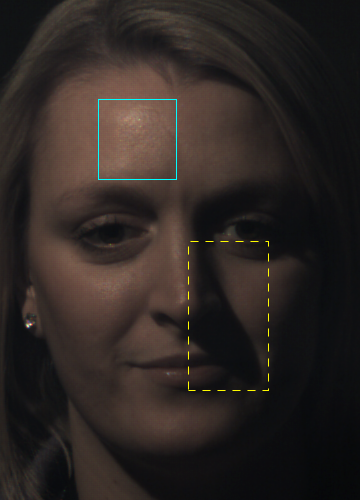
\includegraphics[height=2in]{background/images/photoface2} \hfill
	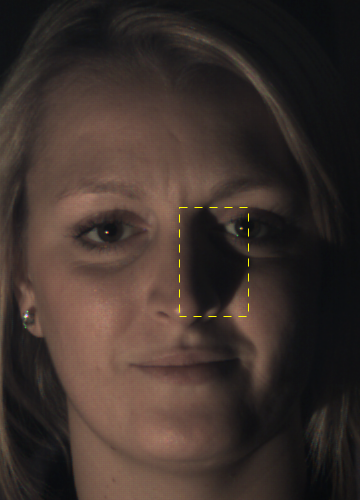
\includegraphics[height=2in]{background/images/photoface3}
	\hspace*{\fill}
	\caption{An example of Photometric Stereo imaging ``in-the-wild'' from
	         the Photoface database~\cite{RefWorks:293}. Notice the cast-shadows
	         (yellow dashed) and specular highlights (cyan solid) present in 
	         the images.}
\label{fig:bg_ps_photoface}
\end{figure}
%%%%%%%%%%%%%%%%%%%%%%%%%%%%%%%%%%%%%%%%

Although PS resolves the ambiguity present in the SfS problem with respect
to the number of inputs, traditional Lambertian PS is still sensitive to
deviations from Lambertian effects in the input images. For faces, this
is particularly evident in the form of cast shadows. For a given pixel that
corresponds to a point on the facial surface, this pixel must have varying
intensity in each of the input images. Practically, this implies that the face
must be lit from a set of reasonably obtuse angles which are prone to causing
cast shadows. An example of both specular highlights and cast shadows that
naturally occur in facial PS imaging is given in \cref{fig:bg_ps_photoface}.
Another issue is that time-multiplexed illumination causes the input
images to lose alignment with one another. If the subject moves at all
during capturing then the input images are not aligned and this breaks
one of the primary assumptions of PS:\@ that each pixel has multiple intensities
of the same surface point with which to compute the normal. An alternative
way to perform Photometric Stereo is
\textit{Multi-spectral Photometric Stereo} (MS-PS). Here MS-PS refers to
using lighting of varying wavelengths in order to simultaneously capture
multiple inputs per pixel. This is sometimes referred to as 
Colour Photometric Stereo~\cite{petrov1987light,woodham1994gradient,%
kontsevich1994reconstruction,hernandez2007non}, 
but there is no hard requirement that the wavelengths are perfectly
interpretable as `colours'~\cite{fyffe2011single} and therefore we refer to this
as multi-spectral. This is also in contrast to other uses of the term multi-
spectral which may refer to the separation of differing reflectance behaviours
within an input image~\cite{nayar1997separation,mallick2005beyond,zickler2008color}.
In contrast to traditional time-multiplexed PS (TM-PS), multi-spectral PS
recovers multiple inputs by assuming that a colour camera CCD has sensors that
are sensitive to at least 3, traditionally red, green and blue (RGB), distinct 
wavelengths. Thus, rather than multiple time multiplexed illuminations from
identical lights, MS-PS assumes multiple spectrally unique illuminations from
multiple directions which contribute differently to each sensor output
of the camera. More precisely, assuming $s$ different sensors within the camera
(typically $s = 3$, RGB), MS-PS is defined by:
%%%%%%%%%%%%%%%%%%%
\begin{equation}\label{eg:bg_ps_lambertian_ms_ps}
	 \min_{\bb{\tilde{N}}} \lVert \bb{C} - \bb{\tilde{N}} \bb{S} \bb{V}^T \rVert_F
\end{equation}
%%%%%%%%%%%%%%%%%%%
where $\bb{\tilde{N}}$ and $\bb{S}$ are as in \cref{eg:bg_ps_lambertian_ls}
and $\bb{C} = {[\bb{c}_1, \ldots, \bb{c}_d]}^T \in \R^{d \times s}$ and 
$\bb{c} = {[c_1, \ldots, c_s]}^T \in \R^{s \times 1}$ are the intensities 
per wavelength in the image. $\bb{V} \in \R^{s \times n}$ is the sensor 
response matrix and the single entry $v_{ij}$:
%%%%%%%%%%%%%%%%%%%
\begin{equation}\label{eg:bg_ps_sensor_response}
	v_{ij} = \int E_j(\lambda) \alpha(\lambda) S_i(\lambda) \; d\lambda
\end{equation}
%%%%%%%%%%%%%%%%%%%
defines the sensor response for the $i$th sensor under the $j$th light for
a specific wavelength of light denoted $\lambda$. Thus $E_j(\lambda)$ is the
spectral distribution of light $j$, $S_i(\lambda)$ is the sensitivity
of sensor $i$ and $\alpha(\lambda)$ is the characteristic chromaticity for the 
given material. Although MS-PS allows for simultaneously illumination of the
face, it requires careful calibration of the sensor response matrix. This
calibration matrix is unique to the illumination set up and face and thus 
calibration must be performed separately for each individual
being captured.

As discussed in \cref{subsec:bg_capture}, PS has been used to collect both
facial reflectance and facial surface databases. Due to the explicit
calibration of lighting conditions and the fact that multiple images are 
required, we largely regard PS as a dedicated capture methodology. Although
there have been efforts to perform PS on less constrained conditions, as in
the Photoface Database~\cite{RefWorks:293}, it still requires calibrated 
lighting and specialised hardware. However, the PS problem can be relaxed by
considering the separation of lighting and surface components as a matrix
factorisation problem. This is called 
\textit{Uncalibrated Photometric Stereo} (U-PS), due to the lack of
requirement for calibrated illumination.
%%%%%%%%%%%%%%%%%%%%%%%%%%%%%%%%%%%%%%%%%%%%%%%%%%%%%%%%%%%%%%%%%%%%%%%%%%%%%%%%
